\section{Local Indexing} \label{sec:local_indexing}

\begin{figure}[b]
    \centering
    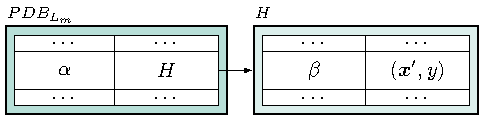
\includegraphics[width=1\linewidth]{tikz/indexing.pdf}
    \caption{Nested indexing in a local pattern database.}
    \label{fig:indexing}
\end{figure}

The local indexing service listens on $C_{L_m}$ for new data points from $D_m$. First, data points are buffered until a defined batch size is released. Subsequently, the batch $X$ is scaled to the range $[-1, 1]$ by applying a feature-wise min-max normalization, given by

\begin{align*}
    \bm{X}' = \frac{\bm{X}-min(\bm{X})}{max(\bm{X}) - min(\bm{X})} \cdot (b - a) + a, \quad
    \setlength\arraycolsep{2pt}
    \begin{array}{lr}
        a = &-1 \\
        b = & 1    
    \end{array}.
\end{align*}

After that, each element $\bm{x}' \in \bm{X}'$ is subject to both a \textit{GRP} $h$ with a global seed for the initialization of the projection plane $\bm{M}$ (see Section \ref{subsec:gaussian_random_projection}) and a non-cryptographic hashing function $g$ (see Section \ref{subsubsec:non-cryptographic-hashes}). The \textit{GRP} clusters the data by mapping similar data points $\bm{x}'$ to the same hash value. The non-cryptographic hashing function on the other hand serves as a mechanism for deduplicating identical $\bm{x}'$. In order to insert a pair $(\bm{x}'_n, y_n) \in D_m$ into the $PDB_{L_m}$, at first two keys $k_\alpha, k_\beta \in K$ are constructed as

\begin{align*}
    k_\alpha(\bm{x}'_n, y_n) &= p_x \doubleplus h(\bm{x}'_n) \doubleplus y_n,\\
    k_\beta(\bm{x}'_n) &= g(\bm{x}'_n),
\end{align*}

where $\doubleplus$ indicates the concatenation operator and $p_x$ describes an arbitrary prefix constant. Secondly, if not already present, a hash table $T_{m_n}$ is created and inserted into the slot $PDB_{L_m}(k_\alpha(\bm{x}'_n, y_n))$. Finally, $(\bm{x}'_n, y_n)$ is hashed into the slot $T_{m_n}(k_\beta(\bm{x}'_n))$. That nested indexing is depicted in Figure \ref{fig:indexing}. Since a particular $h(\bm{x}')$ is a cluster of similar data points, we refer to it as a \textit{region}. Therefore, every region is represented by one or more hash tables $T_{m_n}$, each of them containing data points that belong to the same label. Each execution of that insert operation is executed idempotently, such that the pattern database only returns a response upon the insertion of new data points. For each response, the corresponding region $h(\bm{x}'_n)$ is sent into the local event channel $C_{L_m}$ as an event that indicates a change on a certain cluster within the local pattern database.